\section{Containerization}

\begin{figure}
  \centering
  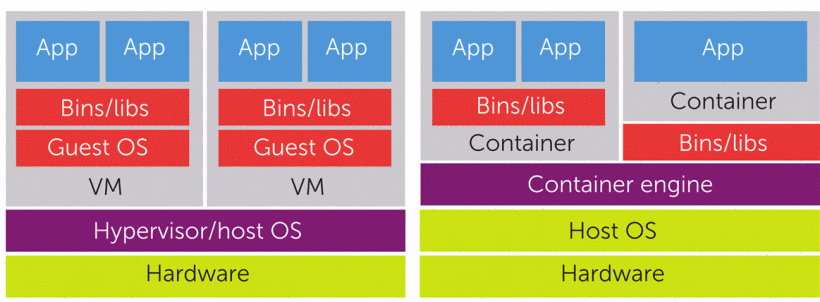
\includegraphics{resources/vm-vs-container.png}
  \caption{
    A comparison between VM and container based virtualization architectures\\
    Source: \citetitle{ieee-containers} \cite{ieee-containers}
  }
  \label{fig:vm-vs-container}
\end{figure}

For a long time VMs have been the standard virtualization technology used in
cloud environments in order to provide virtualized infrastructure with an
abstraction level at the operating system level. While containers are also a
virtualization technique, VMs and containers address different problems. VMs
allow virtual hardware allocation and management, while containers address the
issue of interoperable applications. In the cloud environment (see chapter
\ref{sec:cloud-computing}) VMs focus on the infrastructure layer while
containers are used in the platform layer \cite{ieee-containers}.

While VMs have been used in order to schedule processes as manageable units they
require a file system containing a full operating system. This results in large
memory and storage requirements and slow startup times. In contrast, containers
share their OS with the host they are running on and only hold application code,
runtime, system tools, and system libraries needed for the application (see
figure \ref{fig:vm-vs-container}). This enables interoperability while making
containers lightweight.

Today most containerization technologies are based on the Linux Container (LXC)
technique. LXC facilitates namespace isolation, which allows groups of processes
to be separated. This prevents the (read and write) access to other resources
running on the same host and is used to isolate processes, inter-process
communication, networking, mount points, and kernel and version identifiers.

A container describes a running instance of a container image. While VMs mount
the file root file system in read-write mode (after executing integrity checks),
containers mount the root file system as read-only and utilize union mounts in
order to add a writable file system on top of the read-only root file system.
This allows easier distribution and replacement of images, even for existing
containers.

\subsection{Container Runtime (CR) and Container Manager (CM)}
\label{sec:container-runtime}

\todo[inline]{Use OCI specifications to make this section clearer}
\todo[inline]{Explain container image registry}

Container runtimes are the pieces of software that manage the lifecycle of
containers. Today these runtimes fall mostly fall into two categories, low-level
and high-level runtime. While low-level runtimes like runc or kata are only
responsible for spawning and running containers on the host, high-level runtimes
like containerd or cri-o build on top of low-level runtimes and also manage
container images. In order to differentiate and avoid confusion we will refer to
high-level runtimes as container managers in this thesis.
